\section{並列更新アルゴリズム}\label{section:update}

本節では,後続の操作をブロックしない${\it update\/}$操作を与える.基本的な
アイデアは,zig-zigとzig-zagの両方について,目標節点をその深さの
半分までしか浮上させない半扁平化(semi-splaying)を用いることである(文献
\cite{ST85}の半扁平化は,zig-zigのみが扁平化と異なっていた).$x$を更新対
象の節点とすると,アルゴリズムは以下のようになる.
%
% ここでも左右対称な操作の片方のみを述べる.

\begin{itemize}
% \medskip\noindent (a)
\item[(a)]
空の木に対する挿入は図\ref{figure:update}
(a1)の操作,(空でない)木の根に対する更新は
図\ref{figure:update}(a2)の操作を行なう.

% \begin{adjustvboxheight}
\begin{figure*}[t]
  \centerline {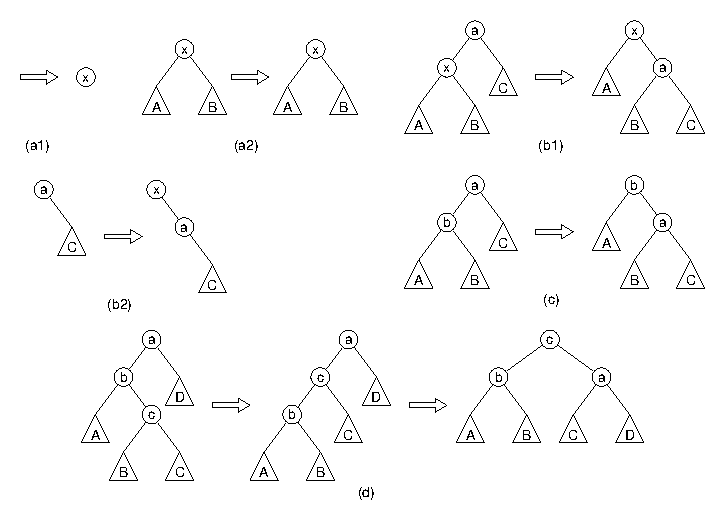
\includegraphics {images/fig3.eps}}
\caption{後続操作をブロックしない更新アルゴリズムの1ステップ}
\label{figure:update}
\end{figure*}
% \end{adjustvboxheight}

% \medskip\noindent (b)
\item[(b)]
zig:
$x$が左部分木の根である場合は図\ref{figure:update}(b1)
の操作,$x$が存在すべき左部分木が空の
場合は図\ref{figure:update}(b2)の操作を行なう.

% \medskip\noindent (c)
\item[(c)]
zig-zig: 図\ref{figure:update}(c)左の木における$x (<b)$の探索では,
枝$ba$の右回転を行なってアクセスしたパスの長さを1短縮する.次は1レベル
(短縮前の長さでは2レベル)下降して,部分木$A$に対して再帰的に探索を行なう.

% \medskip\noindent (d)
\item[(d)]
zig-zag: 図\ref{figure:update}(d)左の木における節点$x$ ($b<x<a$) の
探索では,
枝$cb$の左回転と,できた枝$ca$の右回転を行ない,
アクセスしたパスを1短縮する.
%
% 二つの中側の部分木の適当な方に対して再帰的に探索を行なう.
%
% \noindent
$x=c$ならばこれで探索終了である.$x<c$ならば2レベル(短縮前の長さでは3レ
ベル)下降して$B$の中から$x$を再帰的に
探索する.$x>c$ならば同様に$C$の中から再帰的に探索する.$x\ge c$の場合には
枝$ca$の回転操作を省略することも考えられる.
%
$b$の右部分木が空の場合は,そこに節点$x$を挿入
したあと,上に述べた回転操作を行なう.

\end{itemize}
% \medskip
以上の操作で,アクセスしたパスの長さは最悪でも約$2/3$になる.
%
半分でなくて$2/3$なのは,上記zig-zag操作の性質によるものである.
